% ============================================================
% LLM-BLM 実験 S1：小型株で、決算発表文の読み取りは発表後のドリフトを予測するか（事前登録した検定の結果）
% コンパイル：tectonic -X compile LLM-BLM_実験S1.tex   （XeTeX 系。このフォルダで実行する）
% 数値と表は 図/values.tex・図/tab_*.tex（作成スクリプト/values.py）、図は 図/*.pdf（作成スクリプト/figs.py）。
% どちらも experiments/S1_smallcap_drift/results から作る。本文に数値を手で書かない。
% ============================================================
\documentclass[xelatex,ja=standard,jafont=haranoaji,a4paper,10pt,openany]{bxjsreport}
\setpagelayout*{left=24mm,right=24mm,top=24mm,bottom=26mm,footskip=11mm}

\usepackage{amsmath,amssymb,mathtools,bm}
\usepackage{booktabs,array,multirow,longtable}
\usepackage{graphicx}
\usepackage{adjustbox}
\usepackage{xcolor}
\usepackage{enumitem}
\usepackage{caption}
\usepackage{float}
\usepackage[most]{tcolorbox}
\usepackage[hidelinks,bookmarksnumbered]{hyperref}

\graphicspath{{図/}}
% values.py が results から作る。手で直さない。
\expandafter\def\csname v@commit\endcsname{69a0e12}
\expandafter\def\csname v@npanel\endcsname{38,054}
\expandafter\def\csname v@neval\endcsname{15,997}
\expandafter\def\csname v@nevalgpt\endcsname{7,589}
\expandafter\def\csname v@dry\endcsname{いいえ}
\expandafter\def\csname v@Pcoef\endcsname{$+$76.1}
\expandafter\def\csname v@Pt\endcsname{$+$3.20}
\expandafter\def\csname v@Pp\endcsname{$<$0.001}
\expandafter\def\csname v@Plo\endcsname{$+$29.5}
\expandafter\def\csname v@Phi\endcsname{$+$122.6}
\expandafter\def\csname v@Pn\endcsname{15,174}
\expandafter\def\csname v@Pdates\endcsname{1,384}
\expandafter\def\csname v@Prtwo\endcsname{0.082}
\expandafter\def\csname v@Pperm\endcsname{0.0010}
\expandafter\def\csname v@Pverdict\endcsname{支持}
\expandafter\def\csname v@Rcoef\endcsname{$+$89.9}
\expandafter\def\csname v@Rt\endcsname{$+$3.70}
\expandafter\def\csname v@Rp\endcsname{$<$0.001}
\expandafter\def\csname v@Rlo\endcsname{$+$42.3}
\expandafter\def\csname v@Rhi\endcsname{$+$137.5}
\expandafter\def\csname v@Rn\endcsname{13,164}
\expandafter\def\csname v@Rdates\endcsname{1,171}
\expandafter\def\csname v@Rrtwo\endcsname{0.130}
\expandafter\def\csname v@Ecoef\endcsname{$-$3.1}
\expandafter\def\csname v@Et\endcsname{$-$0.11}
\expandafter\def\csname v@Ep\endcsname{0.543}
\expandafter\def\csname v@Elo\endcsname{$-$59.6}
\expandafter\def\csname v@Ehi\endcsname{$+$53.4}
\expandafter\def\csname v@En\endcsname{15,174}
\expandafter\def\csname v@Edates\endcsname{1,384}
\expandafter\def\csname v@Ertwo\endcsname{0.000}
\expandafter\def\csname v@Mmonths\endcsname{80}
\expandafter\def\csname v@Mexa\endcsname{$+$0.28\%}
\expandafter\def\csname v@Mta\endcsname{$+$1.26}
\expandafter\def\csname v@Mexb\endcsname{$+$0.16\%}
\expandafter\def\csname v@Mtb\endcsname{$+$0.73}
\expandafter\def\csname v@Mexc\endcsname{$+$0.08\%}
\expandafter\def\csname v@Mtc\endcsname{$+$0.38}
\expandafter\def\csname v@Mturn\endcsname{27\%}
\expandafter\def\csname v@Gmonths\endcsname{32}
\expandafter\def\csname v@Gexa\endcsname{$+$0.10\%}
\expandafter\def\csname v@Gta\endcsname{$+$0.38}
\expandafter\def\csname v@Gexb\endcsname{$-$0.04\%}
\expandafter\def\csname v@Gtb\endcsname{$-$0.15}
\expandafter\def\csname v@Gexc\endcsname{$-$0.14\%}
\expandafter\def\csname v@Gtc\endcsname{$-$0.51}
\expandafter\def\csname v@Gturn\endcsname{32\%}
\expandafter\def\csname v@Mtop\endcsname{$+$1.68\%}
\expandafter\def\csname v@Mall\endcsname{$+$1.40\%}
\expandafter\def\csname v@Mstart\endcsname{2020-01}
\expandafter\def\csname v@Mend\endcsname{2026-08}
\expandafter\def\csname v@Gtop\endcsname{$+$1.53\%}
\expandafter\def\csname v@Gall\endcsname{$+$1.42\%}
\expandafter\def\csname v@Gstart\endcsname{2024-01}
\expandafter\def\csname v@Gend\endcsname{2026-08}
\expandafter\def\csname v@dictionarycoefT\endcsname{$-$43.3}
\expandafter\def\csname v@dictionarytT\endcsname{$-$2.08}
\expandafter\def\csname v@finbertcoefT\endcsname{$+$8.6}
\expandafter\def\csname v@finberttT\endcsname{$+$0.40}
\expandafter\def\csname v@finbertftcoefT\endcsname{$+$45.6}
\expandafter\def\csname v@finbertfttT\endcsname{$+$1.96}
\expandafter\def\csname v@chronomidridgecoefT\endcsname{$+$71.5}
\expandafter\def\csname v@chronomidridgetT\endcsname{$+$3.15}
\expandafter\def\csname v@gptcoefS\endcsname{$+$148.9}
\expandafter\def\csname v@gpttS\endcsname{$+$4.21}
\expandafter\def\csname v@gptridgecoefS\endcsname{$+$126.8}
\expandafter\def\csname v@gptridgetS\endcsname{$+$3.45}
\expandafter\def\csname v@chronoridgecoefS\endcsname{$+$119.1}
\expandafter\def\csname v@chronoridgetS\endcsname{$+$3.13}
\expandafter\def\csname v@B2015quarterchronoridge\endcsname{5.078}
\expandafter\def\csname v@B2015quarterchronoridgeex\endcsname{$+$2.8\%}
\expandafter\def\csname v@B2015quarterband\endcsname{3.906}
\expandafter\def\csname v@B2015quarterbandex\endcsname{--}
\expandafter\def\csname v@B2015halfchronoridge\endcsname{4.807}
\expandafter\def\csname v@B2015halfchronoridgeex\endcsname{$+$2.4\%}
\expandafter\def\csname v@B2015halfband\endcsname{3.838}
\expandafter\def\csname v@B2015halfbandex\endcsname{--}
\expandafter\def\csname v@B2015yearchronoridge\endcsname{4.732}
\expandafter\def\csname v@B2015yearchronoridgeex\endcsname{$+$1.6\%}
\expandafter\def\csname v@B2015yearband\endcsname{4.065}
\expandafter\def\csname v@B2015yearbandex\endcsname{--}
\expandafter\def\csname v@B2023quarterchronoridge\endcsname{1.873}
\expandafter\def\csname v@B2023quarterchronoridgeex\endcsname{$+$10.3\%}
\expandafter\def\csname v@B2023quarterfinbertft\endcsname{1.773}
\expandafter\def\csname v@B2023quarterfinbertftex\endcsname{$+$7.8\%}
\expandafter\def\csname v@B2023quartergpt\endcsname{1.761}
\expandafter\def\csname v@B2023quartergptex\endcsname{$+$7.5\%}
\expandafter\def\csname v@B2023quartergptridge\endcsname{1.527}
\expandafter\def\csname v@B2023quartergptridgeex\endcsname{$+$1.3\%}
\expandafter\def\csname v@B2023quarterband\endcsname{1.479}
\expandafter\def\csname v@B2023quarterbandex\endcsname{--}
\expandafter\def\csname v@B2023halfchronoridge\endcsname{1.766}
\expandafter\def\csname v@B2023halfchronoridgeex\endcsname{$+$6.9\%}
\expandafter\def\csname v@B2023halffinbertft\endcsname{1.704}
\expandafter\def\csname v@B2023halffinbertftex\endcsname{$+$5.3\%}
\expandafter\def\csname v@B2023halfgpt\endcsname{1.636}
\expandafter\def\csname v@B2023halfgptex\endcsname{$+$3.5\%}
\expandafter\def\csname v@B2023halfgptridge\endcsname{1.455}
\expandafter\def\csname v@B2023halfgptridgeex\endcsname{$-$1.5\%}
\expandafter\def\csname v@B2023halfband\endcsname{1.508}
\expandafter\def\csname v@B2023halfbandex\endcsname{--}
\expandafter\def\csname v@B2023yearchronoridge\endcsname{1.683}
\expandafter\def\csname v@B2023yearchronoridgeex\endcsname{$+$3.6\%}
\expandafter\def\csname v@B2023yearfinbertft\endcsname{1.874}
\expandafter\def\csname v@B2023yearfinbertftex\endcsname{$+$8.4\%}
\expandafter\def\csname v@B2023yeargpt\endcsname{1.676}
\expandafter\def\csname v@B2023yeargptex\endcsname{$+$3.4\%}
\expandafter\def\csname v@B2023yeargptridge\endcsname{1.470}
\expandafter\def\csname v@B2023yeargptridgeex\endcsname{$-$2.2\%}
\expandafter\def\csname v@B2023yearband\endcsname{1.550}
\expandafter\def\csname v@B2023yearbandex\endcsname{--}
\expandafter\def\csname v@Xdays2260chronoridgec\endcsname{$+$70.8}
\expandafter\def\csname v@Xdays2260chronoridget\endcsname{$+$3.82}
\expandafter\def\csname v@Xdays2260chronoridgen\endcsname{15,177}
\expandafter\def\csname v@Xdays2260finbertftc\endcsname{$+$47.7}
\expandafter\def\csname v@Xdays2260finbertftt\endcsname{$+$2.56}
\expandafter\def\csname v@Xdays2260finbertftn\endcsname{15,177}
\expandafter\def\csname v@Xdays2260dictionaryc\endcsname{$-$15.6}
\expandafter\def\csname v@Xdays2260dictionaryt\endcsname{$-$0.95}
\expandafter\def\csname v@Xdays2260dictionaryn\endcsname{15,177}
\expandafter\def\csname v@Xdays2260gptgptc\endcsname{$+$79.9}
\expandafter\def\csname v@Xdays2260gptgptt\endcsname{$+$2.64}
\expandafter\def\csname v@Xdays2260gptgptn\endcsname{6,851}
\expandafter\def\csname v@Xdays2260gptgptridgec\endcsname{$+$63.5}
\expandafter\def\csname v@Xdays2260gptgptridget\endcsname{$+$2.02}
\expandafter\def\csname v@Xdays2260gptgptridgen\endcsname{6,851}
\expandafter\def\csname v@Xdays2260gptchronoridgec\endcsname{$+$76.6}
\expandafter\def\csname v@Xdays2260gptchronoridget\endcsname{$+$2.56}
\expandafter\def\csname v@Xdays2260gptchronoridgen\endcsname{6,851}
\expandafter\def\csname v@Xplusmomentumchronoridgec\endcsname{$+$92.5}
\expandafter\def\csname v@Xplusmomentumchronoridget\endcsname{$+$3.81}
\expandafter\def\csname v@Xplusmomentumchronoridgen\endcsname{15,174}
\expandafter\def\csname v@Xplusmomentumfinbertftc\endcsname{$+$56.5}
\expandafter\def\csname v@Xplusmomentumfinbertftt\endcsname{$+$2.35}
\expandafter\def\csname v@Xplusmomentumfinbertftn\endcsname{15,174}
\expandafter\def\csname v@Xplusmomentumgptgptc\endcsname{$+$181.4}
\expandafter\def\csname v@Xplusmomentumgptgptt\endcsname{$+$4.83}
\expandafter\def\csname v@Xplusmomentumgptgptn\endcsname{6,849}
\expandafter\def\csname v@Xplusmomentumgptgptridgec\endcsname{$+$157.2}
\expandafter\def\csname v@Xplusmomentumgptgptridget\endcsname{$+$4.14}
\expandafter\def\csname v@Xplusmomentumgptgptridgen\endcsname{6,849}
\expandafter\def\csname v@Xplusmomentumgptchronoridgec\endcsname{$+$150.6}
\expandafter\def\csname v@Xplusmomentumgptchronoridget\endcsname{$+$3.88}
\expandafter\def\csname v@Xplusmomentumgptchronoridgen\endcsname{6,849}
\expandafter\def\csname v@Xbysizesmallerc\endcsname{$+$81.3}
\expandafter\def\csname v@Xbysizesmallert\endcsname{$+$2.30}
\expandafter\def\csname v@Xbysizesmallern\endcsname{7,571}
\expandafter\def\csname v@Xbysizelargerc\endcsname{$+$66.7}
\expandafter\def\csname v@Xbysizelargert\endcsname{$+$2.41}
\expandafter\def\csname v@Xbysizelargern\endcsname{7,603}
\expandafter\def\csname v@Xcorrchronoridge\endcsname{0.29}
\expandafter\def\csname v@Xcorrfinbertft\endcsname{0.23}
\expandafter\def\csname v@Xcorrgpt\endcsname{0.28}
\expandafter\def\csname v@Xcorrgptridge\endcsname{0.28}

\newcommand{\V}[1]{\ifcsname v@#1\endcsname\csname v@#1\endcsname\else\textbf{??#1??}\fi}
\newcommand{\tabin}[1]{\adjustbox{max width=\linewidth}{\input{図/tab_#1.tex}}}

\definecolor{c1}{HTML}{2A78D6}
\definecolor{c2}{HTML}{EB6834}
\definecolor{c3}{HTML}{1BAF7A}
\definecolor{c4}{HTML}{EDA100}
\definecolor{ink2}{HTML}{52514E}
\definecolor{soft1}{HTML}{E4EEF9}
\definecolor{soft2}{HTML}{FBEEDF}
\definecolor{soft5}{HTML}{FDF3DA}

\newcommand{\code}[1]{\texttt{#1}}
\newcommand{\SP}{S\&P500}
\newcommand{\figref}[1]{図~\ref{#1}}
\newcommand{\tabref}[1]{表~\ref{#1}}
\newcommand{\chapref}[1]{第~\ref{#1}~章}

\setlist[itemize]{leftmargin=1.6em,itemsep=0.2em,topsep=0.4em}
\setlist[enumerate]{leftmargin=1.8em,itemsep=0.2em,topsep=0.4em}
\captionsetup{font=small,labelfont=bf,skip=6pt}
\renewcommand{\arraystretch}{1.2}

\makeatletter
\def\@makechapterhead#1{\vspace*{0.3\Cvs}{\parindent\z@\raggedright\normalfont
  \ifnum\c@secnumdepth>\m@ne\if@mainmatter{\Large\headfont\@chapapp\thechapter\@chappos}\par\nobreak\vskip0.4\Cvs\fi\fi
  \interlinepenalty\@M\LARGE\headfont #1\par\nobreak\vskip 1.5\Cvs}}
\def\@makeschapterhead#1{\vspace*{0.3\Cvs}{\parindent\z@\raggedright\normalfont
  \interlinepenalty\@M\LARGE\headfont #1\par\nobreak\vskip 1.5\Cvs}}
\makeatother

\newtcolorbox{keybox}[1][要点]{enhanced,breakable,colback=soft1,colframe=c1,boxrule=0.5pt,arc=2pt,
  left=8pt,right=8pt,top=6pt,bottom=6pt,title={#1},fonttitle=\sffamily\bfseries\small,coltitle=white}
\newtcolorbox{notebox}[1][注意]{enhanced,breakable,colback=soft2,colframe=c2,boxrule=0.5pt,arc=2pt,
  left=8pt,right=8pt,top=6pt,bottom=6pt,title={#1},fonttitle=\sffamily\bfseries\small,coltitle=white}

\title{LLM-BLM 実験 S1\\[6pt]
  \large 小型株で、決算発表文の読み取りは\\発表後のドリフトを予測するか}
\author{実験の報告書（事前登録した検定の結果）}
\date{2026 年 10 月 24 日}

\begin{document}
\maketitle

\chapter*{概要}
\addcontentsline{toc}{chapter}{概要}

\SP{} では、LLM の決算発表文の読み取りは発表の当日に株価に入りきり、翌日以降のドリフトは予測しなかった（実験 2・3・8）。そこで、注目の低い小型株（浮動株時価総額で 1,001〜3,000 位、1,000 社）で、読み取りが発表の後 2〜60 取引日のドリフトを予測するかを、事前登録して 1 回だけ確かめた。

\begin{keybox}[要点]
\begin{itemize}
\item \textbf{主な検定は支持された}。ChronoGPT（2015 年版）のベクトルに、2 日の反応を正解にしたリッジを当てた点数が 1 標準偏差高い発表は、2 日の反応・SUE などを統制した後、2〜60 日の IWM との超過リターンが \V{Pcoef} bp 高かった（$t$ = \V{Pt}、置換の片側 $p$ \V{Pperm}、発表 \V{Pn} 件）。2021 年以降だけでも \V{Rcoef} bp（$t$ = \V{Rt}）。
\item \textbf{gpt-4o-mini}（2024 年以降）は、学習なしで \V{gptcoefS} bp（$t$ = \V{gpttS}）、重みを学習して \V{gptridgecoefS} bp（$t$ = \V{gptridgetS}）と、さらに強かった。学習なしの辞書は負、FinBERT はゼロだった。
\item \textbf{ドリフトは主に 22〜60 日目}に出ていた（ChronoGPT）。過去 1 年のモメンタムを統制に加えても消えず、規模の大小のどちらの半分でも見られた（事前登録の後の探索）。
\item \textbf{取引の成績にはならなかった}。浮動株時価総額で加重した上位 20\% の月次のポートフォリオは、片道 0.3\% の費用の後で、範囲の全社を月 \V{Mexb} 上回ったが、有意ではなかった（$t$ = \V{Mtb}、\V{Mmonths} か月）。
\item \textbf{BLM の資産の推移}（追記 1、検定はしない）：ChronoGPT＋リッジの見通しの BLM は、2015 年末からの四半期ごとのリバランスで、最終の値が \V{B2015quarterchronoridge}、比べる相手（範囲の全社、浮動株時価総額で加重）が \V{B2015quarterband}（年率の差 \V{B2015quarterchronoridgeex}）だった。半年・1 年ごとでも、2023 年末からでも上回った。ただし差の多くは 2023 年以降に開き、資産の水準は生存者バイアスで高く出ている。

\item \textbf{注意}：標本は今も上場している会社だけである（生存者バイアス）。収益性・アナリストの予想の修正は統制していない。結果は 1 回の実行のものである。
\end{itemize}
\end{keybox}


\setcounter{tocdepth}{1}
{\small\tableofcontents}

% ============================================================
\chapter{目的}\label{ch:purpose}

\section{これまでの結果}

\SP{} の決算発表文では、LLM（gpt-4o-mini）・FinBERT・ChronoGPT の読み取りは、発表をはさむ 2 日の株価の反応を強く説明した（実験 2〜5・11）。しかし、翌日以降のドリフトは有意に予測しなかった（実験 2・3・8）。情報は発表の当日に株価に入りきっていた。

\section{問い}

Hong・Stein（1999）、Akbas ほか（2017）などによれば、反応の遅れは注目されていない銘柄に集中する。そこで、注目の低い小型株で、次の問いを確かめた。

\begin{keybox}[問い]
注目の低い小型株では、決算発表文の読み取りが、発表後 2〜60 取引日の超過リターン（ドリフト）を予測するか。
\end{keybox}

あわせて、利用者の依頼（2026-10-23）に従い、FinBERT・ChronoGPT の学習あり、gpt-4o-mini、gpt-4o-mini の学習あり（点数に重みを学習）を比べ、四半期・半年・1 年ごとにリバランスする BLM の資産の推移を作った（事前登録の追記 1）。

% ============================================================
\chapter{事前登録}\label{ch:prereg}

検定の仮説・データ・変数・方法・判定の基準は、\code{experiments/S1\_smallcap\_drift/preregistration.md} に書き、実行するコード（\code{run.py}・\code{blm\_paths.py}）と同じコミットで固定してから、1 回だけ実行した。株価の反応は、それまで一度も計算していない（\code{--dry} は、株価の代わりに乱数を入れて動作だけを確かめたもの）。実行に使ったコミットは \code{\V{commit}}（\code{results/summary.json} に記録）。

\begin{itemize}
\item \textbf{主な検定 P}：2020 年以降に提出され、提出日に小型株の範囲（浮動株時価総額の 1,001〜3,000 位）にいた会社の発表で、2〜60 取引日の IWM との超過リターン（\code{abn\_drift\_2\_60}）を、\code{chrono\_ridge}（ChronoGPT 2015 年版の最後の層の平均のベクトルに、四半期ごとのリッジで 2 日の反応を学習）と統制・固定効果で回帰した係数が正か。
\item \textbf{判定}：片側 $t$ の $p < 0.05$、かつ、同じ反応日の中で点数を 1,000 回入れ替える置換の片側 $p < 0.05$ なら「支持」。
\item \textbf{副次}（判定には使わない）：ほかの点数のドリフトの回帰（2 つの族でそれぞれ Holm の補正）、2 つの期間 × 3 つの目的変数の比較の表、時価総額加重との対決（毎月）、2021 年以降の頑健性。
\item \textbf{追記 1}（どの株価の反応も計算する前に追加）：BLM の資産の推移。検定はせず、報告だけする。
\item \textbf{探索}：ドリフトを正解にして学習したリッジ（\code{chrono\_ridge\_drift}）。
\end{itemize}

% ============================================================
\chapter{データと変数}\label{ch:data}

\section{標本}

\begin{itemize}
\item \code{data/smallcap.sqlite} の 1,000 社（いま上場している会社。生き残った会社だけ）の決算発表文（8-K Item 2.02 の EX-99）。データの作り方と生存者バイアスの見積もりは、「LLM-BLM 小型株のデータ」の報告書にある。
\item 2015 年以降の発表のうち、点数と反応の窓がそろうもの：\V{npanel} 件。
\item 評価する発表（2020 年以降、範囲の中）：\V{neval} 件。そのうち gpt-4o-mini の点数がそろう 2024 年以降の発表：\V{nevalgpt} 件。
\item 2015〜2019 年の発表は、学習にだけ使った。
\end{itemize}

\section{目的変数}

すべて IWM（Russell 2000 の ETF）との差。上下 1\% で丸めた（評価する標本の中で）。

\begin{itemize}
\item 主：\code{abn\_drift\_2\_60}（反応日を day 0 として、2〜60 取引日目）
\item 副：\code{abn\_r\_0\_1}（day 0 の前日の終値から day 1 の終値まで、2 取引日の反応）、\code{abn\_drift\_2\_21}
\end{itemize}

\section{統制}

SUE、売上の驚き（欠けは 0 で埋めて欠けの印を足す）、\code{abn\_pre}（$-21$〜$-1$ 日）、\code{log\_float}、業種（SIC の上 2 桁）と年・四半期の固定効果。ドリフトの回帰には \code{abn\_r\_0\_1} も統制に入れた（市場が 2 日で反応した分を超えるかを見るため）。標準誤差は反応日ごとにまとめた。

\section{点数}

\begin{table}[H]
\centering\small
\caption{比べた点数（評価する標本の中で標準化）}
\label{tab:scores}
\begin{tabular}{@{}lp{0.62\linewidth}l@{}}
\toprule
列 & 中身 & 学習 \\
\midrule
\code{dictionary} & Loughran--McDonald の net tone & なし \\
\code{finbert} & FinBERT（先頭 200 文の平均） & なし \\
\code{finbert\_ft} & 実験 4 と同じ設定の FinBERT の追加学習（2020 年より前に窓が閉じた発表の 2 日の反応で学習） & 2 日の反応 \\
\code{chrono\_ridge} & ChronoGPT 2015 年版、元の文章の最後の層の平均に、四半期ごとのリッジ（主） & 2 日の反応 \\
\code{chrono\_mid\_ridge} & ChronoGPT 2015 年版、掃除した文章の 26 層目の平均に、同じリッジ & 2 日の反応 \\
\code{gpt} & gpt-4o-mini（H06 の質問、温度 0）の語調＋見通し＋ガイダンス & なし \\
\code{gpt\_ridge} & gpt-4o-mini の 14 の項目に、同じ四半期ごとのリッジ & 2 日の反応 \\
\bottomrule
\end{tabular}
\end{table}

学習ありのモデルは、どれも 2 日の反応を正解にして学習した（読み取りの強さを学ぶ）。ドリフトの検定では、その点数が反応の向きに遅れて動く分を予測するかを見る。リッジの学習は、その四半期が始まる前に 2 日の窓が閉じた発表だけを使った。

% ============================================================
% 結果の章（数値は 図/values.tex と 図/tab_*.tex から。手で書かない）

% ============================================================
\chapter{主な検定}\label{ch:primary}

\begin{table}[H]
\centering\small
\caption{主な検定 P：2020 年以降・範囲の中の発表で、2〜60 取引日のドリフトを \code{chrono\_ridge} と統制・固定効果で回帰した結果}
\label{tab:primary}
\begin{tabular}{@{}lr@{}}
\toprule
点数が 1 標準偏差高いときのドリフトの差 & \V{Pcoef} bp \\
95\% 信頼区間 & [\V{Plo}, \V{Phi}] bp \\
$t$（反応日ごとにまとめた標準誤差） & \V{Pt} \\
片側 $p$ & \V{Pp} \\
置換（同じ反応日の中で 1,000 回）の片側 $p$ & \V{Pperm} \\
発表の数（反応日の数） & \V{Pn}（\V{Pdates}） \\
決定係数の増分 & \V{Prtwo} ポイント \\
\midrule
判定 & \textbf{\V{Pverdict}} \\
\bottomrule
\end{tabular}
\end{table}

\begin{keybox}[結果]
事前登録の判定の基準（片側 $t$ の $p < 0.05$、かつ置換の片側 $p < 0.05$）を両方とも満たし、仮説は\textbf{支持}された。ChronoGPT＋リッジの点数が 1 標準偏差高い発表は、発表をはさむ 2 日の反応・SUE・売上の驚き・発表の前の値動き・規模・業種と時期の固定効果を統制したうえで、その後 2〜60 取引日の IWM との超過リターンが平均 \V{Pcoef} bp 高かった。置換の $p$ の \V{Pperm} は、1,000 回の置換のどれも実際の係数を超えなかったことを示す（1,000 回の置換で出せる最小の値）。
\end{keybox}

\begin{itemize}
\item \textbf{大きさ}：1 標準偏差あたり約 0.8\% は、60 取引日（約 3 か月）の超過リターンとしては小さくない。ただし決定係数の増分は \V{Prtwo} ポイントで、個々の発表のドリフトの変動のごく一部しか説明しない。一つ一つの発表の予測は外れることが多い。
\item \textbf{2021 年以降}（生存者バイアスの小さい期間、事前登録の頑健性）：係数 \V{Rcoef} bp（$t$ = \V{Rt}、片側 $p$ \V{Rp}、発表 \V{Rn} 件）。同じ向きで、やや大きい。
\end{itemize}

% ============================================================
\chapter{副次の検定と比較}\label{ch:secondary}

\section{ほかの点数のドリフト}

\begin{table}[H]
\centering\small
\caption{副次の検定：2〜60 日のドリフトの回帰（族ごとに Holm の補正。判定には使わない）}
\label{tab:secondary}
\tabin{secondary}
\end{table}

\begin{itemize}
\item \textbf{学習ありの点数}は、どれも正の係数を持った。ChronoGPT の 26 層目（\code{chrono\_mid\_ridge}）は Holm の補正の後も有意、FinBERT の追加学習（\code{finbert\_ft}）は補正の前は 5\% で有意、補正の後は 10\% の水準だった。
\item \textbf{学習なしの点数}のうち、辞書は負（$t$ は約 $-2$）、FinBERT はほぼゼロだった。
\item \textbf{gpt-4o-mini の期間}（2024 年以降）では、学習なしの gpt-4o-mini（語調＋見通し＋ガイダンス）が最も大きく、重みを学習したもの、ChronoGPT＋リッジも、どれも Holm の補正の後に有意だった。
\end{itemize}

\section{比較の表}

\begin{table}[H]
\centering\small
\caption{2020 年以降：係数（bp/SD）と、括弧の中は $t$}
\label{tab:compare2020}
\tabin{compare_2020}
\end{table}

\begin{table}[H]
\centering\small
\caption{2024 年以降（gpt-4o-mini の点数がそろう発表）：係数（bp/SD）と、括弧の中は $t$}
\label{tab:compare2024}
\tabin{compare_2024}
\end{table}

\begin{figure}[H]
\centering
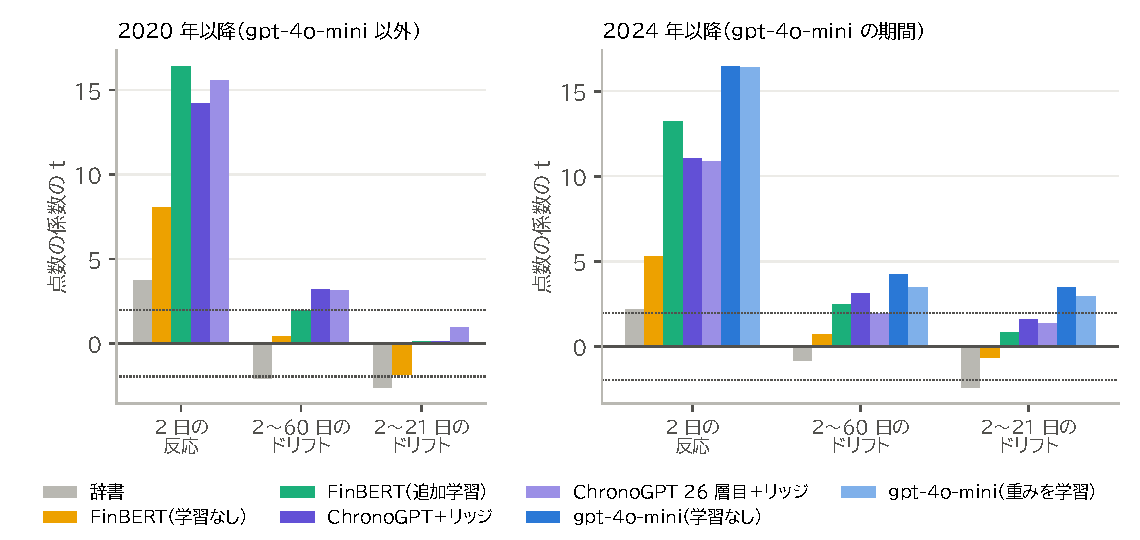
\includegraphics[width=\linewidth]{compare.pdf}
\caption{点数の係数の $t$。点線は $\pm 1.96$。}
\label{fig:compare}
\end{figure}

\begin{itemize}
\item \textbf{2 日の反応}は、どの点数でも強く説明できた。\SP{} の実験と同じで、学習ありのモデル（FinBERT の追加学習、ChronoGPT＋リッジ）と gpt-4o-mini が特に強い。
\item \textbf{2〜21 日}では、ChronoGPT＋リッジの係数はほぼゼロで、gpt-4o-mini（2024 年以降）だけが有意に正だった。辞書は負だった。
\item つまり、ChronoGPT＋リッジの 2〜60 日のドリフトは、主に \textbf{22〜60 日目}に生じている（\ref{sec:explore} 節で確かめた）。
\end{itemize}

% ============================================================
\chapter{時価総額加重との対決}\label{ch:portfolio}

事前登録の副次の 4：毎月末、範囲の中の会社のうち、直近 92 日以内の最新の発表の点数の上位 20\% を浮動株時価総額で加重したポートフォリオと、範囲の全社を浮動株時価総額で加重したもの（比べる相手）を比べた。

\begin{table}[H]
\centering\small
\caption{月次の超過リターン（上位 20\% − 範囲の全社）と Newey--West の $t$（ラグ 3）}
\label{tab:portfolio}
\begin{tabular}{@{}lrrrrrr@{}}
\toprule
 & \multicolumn{2}{c}{費用 0\%} & \multicolumn{2}{c}{片道 0.3\%} & \multicolumn{2}{c}{片道 0.5\%} \\
\cmidrule(lr){2-3}\cmidrule(lr){4-5}\cmidrule(lr){6-7}
 & 月次 & $t$ & 月次 & $t$ & 月次 & $t$ \\
\midrule
ChronoGPT＋リッジ（\V{Mstart}〜\V{Mend}、\V{Mmonths} か月） & \V{Mexa} & \V{Mta} & \V{Mexb} & \V{Mtb} & \V{Mexc} & \V{Mtc} \\
gpt-4o-mini（重みを学習、\V{Gstart}〜\V{Gend}、\V{Gmonths} か月） & \V{Gexa} & \V{Gta} & \V{Gexb} & \V{Gtb} & \V{Gexc} & \V{Gtc} \\
\bottomrule
\end{tabular}
\end{table}

\begin{figure}[H]
\centering
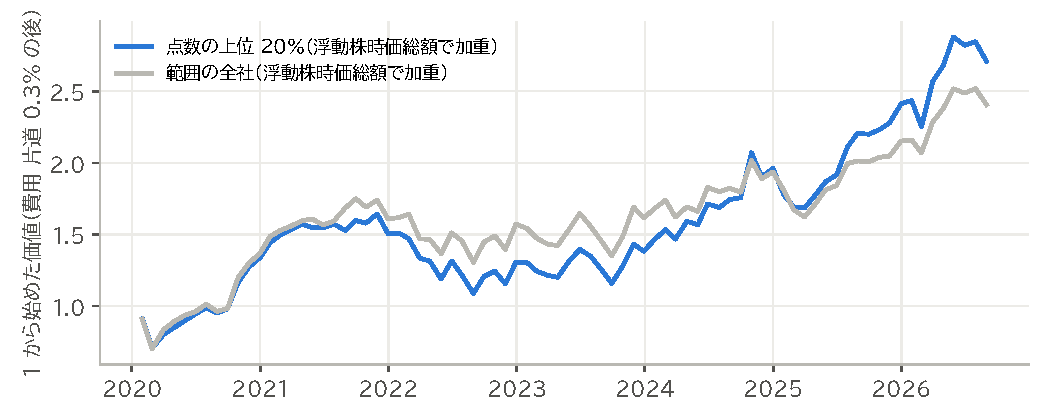
\includegraphics[width=\linewidth]{portfolio.pdf}
\caption{ChronoGPT＋リッジの上位 20\% と、範囲の全社（2020 年 1 月を 1、片道 0.3\% の費用の後）。}
\label{fig:portfolio}
\end{figure}

\begin{figure}[H]
\centering
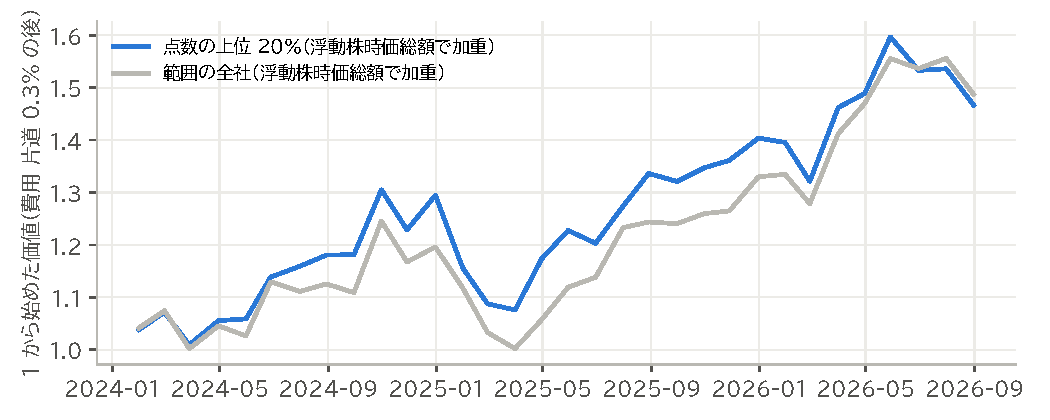
\includegraphics[width=\linewidth]{portfolio_gpt.pdf}
\caption{gpt-4o-mini（重みを学習）の上位 20\% と、範囲の全社（2024 年 1 月を 1、片道 0.3\% の費用の後）。}
\label{fig:portfoliogpt}
\end{figure}

\begin{itemize}
\item ChronoGPT＋リッジの上位 20\% は、費用の前で月 \V{Mexa}、片道 0.3\% の費用の後で月 \V{Mexb}、比べる相手を上回ったが、有意ではなかった（$t$ = \V{Mtb}）。上位 20\% の月の回転率は平均 \V{Mturn}。
\item gpt-4o-mini（重みを学習）は、V{Gmonths} か月と短く、費用の後はほぼゼロだった。
\item 回帰で見えた予測の力（\chapref{ch:primary}）が、浮動株時価総額で加重した月次のポートフォリオの差として、有意に現れるほどの大きさではなかった。回帰は発表を等しく扱い、業種と時期の影響を除くが、ポートフォリオは規模で加重し、市場全体の変動の中で比べる。
\item 両方のポートフォリオの月次の平均リターン（上位 20\% が \V{Mtop}、範囲の全社が \V{Mall}）は、今も上場している会社だけを選んだ生存者バイアスで高く出ている。意味があるのは差だけである。
\end{itemize}

% ============================================================
% BLM の資産の推移（事前登録の追記 1。検定はせず報告だけ）
\chapter{BLM の資産の推移}\label{ch:blm}

事前登録の追記 1（どの株価の反応も計算する前に追加）：四半期（3・6・9・12 月）・半年（6・12 月）・1 年（12 月）ごとにリバランスする BLM の比率で、2015 年 12 月末と 2023 年 12 月末をそれぞれ 1 とした資産の推移を作った（\code{blm\_paths.py}）。

\begin{itemize}
\item 範囲：各リバランスの日に小型株の範囲にいて、直近 252 日のうち 126 日以上の株価がある会社。
\item 見通し：その日以前に反応日がある、直近 92 日以内の最新の発表の点数を正規スコアにした。BLM は実験 7・9 と同じ形（$\delta = 2.5$、$\tau = 0.025$、He--Litterman の $\Omega$、IC $= 0.05$）で、見通しの大きさは保有期間に合わせた（日次で IC × $\sigma_{\text{日}}$ × $z / \sqrt{h}$）。共分散は直近 252 日の Ledoit--Wolf。事前の TE の上限は年 3\%（校正しない）。
\item 比べる相手：同じ範囲を浮動株時価総額で加重したもの。両方から、売買した額の片道 0.3\% を引いた。
\item \textbf{検定はしない}（事前登録の通り、報告だけ）。
\end{itemize}

\section{2015 年末から}

\begin{table}[H]
\centering\small
\caption{2015 年 12 月末を 1 とした資産の推移（2026 年 9 月末まで）。年率と相手との差は年率、実現の TE は年率、回転率はリバランス 1 回あたり}
\label{tab:blm2015}
\tabin{blm_2015}
\end{table}

\begin{figure}[H]
\centering
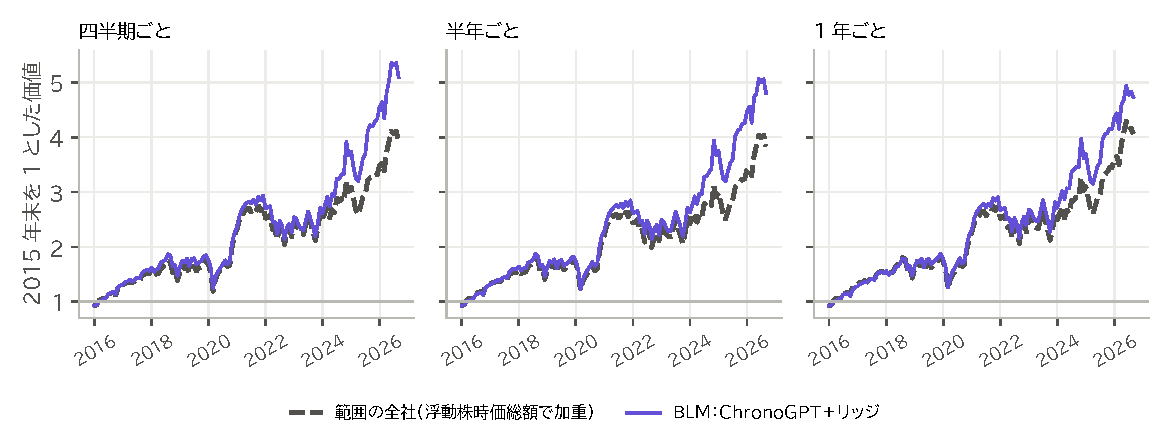
\includegraphics[width=\linewidth]{blm_2015.pdf}
\caption{2015 年末を 1 とした推移。BLM は ChronoGPT＋リッジの見通し。}
\label{fig:blm2015}
\end{figure}

\section{2023 年末から}

\begin{table}[H]
\centering\small
\caption{2023 年 12 月末を 1 とした資産の推移（2026 年 9 月末まで、約 2 年 9 か月）}
\label{tab:blm2023}
\tabin{blm_2023}
\end{table}

\begin{figure}[H]
\centering
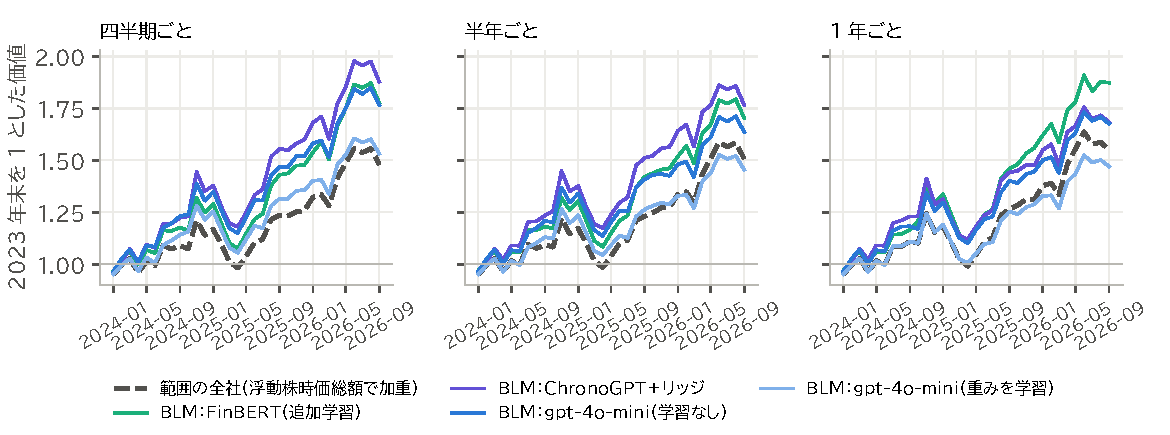
\includegraphics[width=\linewidth]{blm_2023.pdf}
\caption{2023 年末を 1 とした推移。gpt-4o-mini（重みを学習）は 2024 年の第 1 四半期から点数があり、それ以前の日は見通しなし（範囲の比率）。}
\label{fig:blm2023}
\end{figure}

\section{読み方}

\begin{itemize}
\item \textbf{2015 年末から}：ChronoGPT＋リッジの BLM は、3 つのリバランスの頻度のどれでも、比べる相手を年率で上回った（四半期 \V{B2015quarterchronoridgeex}、半年 \V{B2015halfchronoridgeex}、1 年 \V{B2015yearchronoridgeex}）。最終の値は、四半期で \V{B2015quarterchronoridge}、比べる相手は \V{B2015quarterband}。ただし、\figref{fig:blm2015} のとおり、差の多くは 2023 年以降に開いた。2016〜2022 年は、ほぼ同じ動きだった。
\item \textbf{2023 年末から}：ChronoGPT＋リッジ、FinBERT（追加学習）、gpt-4o-mini（学習なし）の BLM は、どの頻度でも比べる相手を上回った。gpt-4o-mini（重みを学習）は、四半期ではわずかに上回り、半年・1 年では下回った。期間が約 2 年 9 か月と短く、1 年ごとのリバランスは 3 回しかない。
\item \textbf{資産の水準}は、2 本とも生存者バイアスで高く出ている（比べる相手の年率が 13〜17\%）。特に 2015 年からの推移は、範囲の会社の約半分が欠ける時期を含む。意味があるのは、同じ会社の範囲での 2 本の差である。
\item \textbf{実現の TE} は年 3〜7\% 程度で、多くは事前の上限（3\%）を超えた。事前の TE を校正しなかったこと（事前登録で決めた）と、最適化の多くの回で解の精度が「不正確」（\code{optimal\_inaccurate}）と報告されたことによる。不正確と報告された解も、そのまま使った（\code{results/blm\_paths.json} の \code{status}）。
\item \textbf{回帰との関係}：主な検定の予測の力（\chapref{ch:primary}）は、BLM の小さな傾き（TE 数\%）の中で、比べる相手との差として現れた。一方、規模で加重した上位 20\% の月次のポートフォリオ（\chapref{ch:portfolio}）では、有意な差にならなかった。どちらも 1 回の実行の結果であり、BLM の差は検定していない。
\end{itemize}


% ============================================================
\chapter{探索}\label{ch:explore}

\section{事前登録した探索：ドリフトを正解に学習したリッジ}

同じ ChronoGPT のベクトルのリッジを、2 日の反応ではなく 2〜60 日のドリフト（窓が閉じたものだけ）を正解にして学習すると、係数は \V{Ecoef} bp（$t$ = \V{Et}）で、予測の力はなかった。ドリフトはばらつきが大きく、それを直接に学習するには標本が足りない。2 日の反応で「読み取りの強さ」を学び、それがドリフトを予測するかを見る事前登録の設計（主な検定）のほうが、うまくいった。

\section{事前登録の後の探索}\label{sec:explore}

以下は、主な検定の結果を見た後に追加した分析で、\textbf{事前登録にない}。コードは \code{explore.py}、結果は \code{results/explore.json}（どちらも \code{experiments/S1\_smallcap\_drift/} の下）。置換の検定はしていない。試した分析はここに書いたものだけだが、これらを結論の根拠にはしない。

\subsection{点数の 5 分位}

\begin{table}[H]
\centering\small
\caption{点数の 5 分位ごとの、IWM との超過リターンの平均（bp、上下 1\% で丸めた。統制なし）}
\label{tab:quintiles}
\tabin{quintiles}
\end{table}

ChronoGPT＋リッジでは、2〜21 日の差は小さく、22〜60 日に上位と下位の差が開く。gpt-4o-mini では 2〜21 日にも差がある。どちらも上位 2 つの分位が高く、下位が低い。

\subsection{22〜60 日だけの窓・モメンタム・規模}

\begin{table}[H]
\centering\small
\caption{事前登録の後の探索の回帰（係数 bp/SD、括弧の中は $t$。統制と固定効果は主な検定と同じ）}
\label{tab:explore}
\begin{tabular}{@{}lll@{}}
\toprule
分析 & 点数 & 結果 \\
\midrule
22〜60 日だけの窓（2020 年以降） & ChronoGPT＋リッジ & \V{Xdays2260chronoridgec}（\V{Xdays2260chronoridget}） \\
 & FinBERT（追加学習） & \V{Xdays2260finbertftc}（\V{Xdays2260finbertftt}） \\
 & 辞書 & \V{Xdays2260dictionaryc}（\V{Xdays2260dictionaryt}） \\
22〜60 日だけの窓（2024 年以降） & gpt-4o-mini（学習なし） & \V{Xdays2260gptgptc}（\V{Xdays2260gptgptt}） \\
 & gpt-4o-mini（重みを学習） & \V{Xdays2260gptgptridgec}（\V{Xdays2260gptgptridget}） \\
\midrule
過去 1 年のモメンタムを統制に追加（2〜60 日） & ChronoGPT＋リッジ & \V{Xplusmomentumchronoridgec}（\V{Xplusmomentumchronoridget}） \\
 & FinBERT（追加学習） & \V{Xplusmomentumfinbertftc}（\V{Xplusmomentumfinbertftt}） \\
 & gpt-4o-mini（学習なし、2024 年以降） & \V{Xplusmomentumgptgptc}（\V{Xplusmomentumgptgptt}） \\
 & gpt-4o-mini（重みを学習、2024 年以降） & \V{Xplusmomentumgptgptridgec}（\V{Xplusmomentumgptgptridget}） \\
\midrule
規模で 2 つに分ける（2〜60 日） & 浮動株時価総額の小さい半分 & \V{Xbysizesmallerc}（\V{Xbysizesmallert}） \\
 & 大きい半分 & \V{Xbysizelargerc}（\V{Xbysizelargert}） \\
\bottomrule
\end{tabular}
\end{table}

\begin{itemize}
\item \textbf{22〜60 日}：ChronoGPT＋リッジのドリフトは、この窓だけでも有意に正だった。
\item \textbf{モメンタム}：点数は過去 1 年の超過リターン（$-251$〜$-22$ 日）と正の順位相関（ChronoGPT＋リッジで \V{Xcorrchronoridge}、gpt-4o-mini で \V{Xcorrgpt}）を持つ。しかし、それを統制に加えても係数は小さくならず、むしろ大きくなった。点数のドリフトの予測は、既知のモメンタムの言い換えではない。
\item \textbf{規模}：浮動株時価総額の小さい半分と大きい半分の両方で、同じ向きに有意だった。小型株の範囲の中で、特に極めて小さな株だけに依存しているわけではない。
\end{itemize}

% ============================================================
\chapter{解釈}\label{ch:interpret}

\section{何が分かったか}

\begin{enumerate}
\item \textbf{小型株では、決算発表文の読み取りが、発表の後のドリフトを予測した}。\SP{} では見られなかった（実験 2・3・8）。注目の低い銘柄で反応が遅れるという Hong・Stein（1999）、Hong・Lim・Stein（2000）、Akbas ほかの考え方と整合的である。数値の驚き（SUE）を統制しても残るので、文章でしか分からない情報がゆっくり価格に入っている、という PEAD.txt（Meursault ほか）の結果とも合う。
\item \textbf{学習ありの読み取りが効いた}。2 日の反応で学習した ChronoGPT・FinBERT のリッジや追加学習は正、学習なしの辞書は負、FinBERT はゼロだった。gpt-4o-mini は学習なしでも強かった。「市場がその日に強く反応した読み取り」ほど、その後も同じ向きに動く。
\item \textbf{ドリフトは 22〜60 日目に多い}（ChronoGPT＋リッジ）。反応の不足の典型的な形（発表の直後に続きが出る）とは少し違う。次の決算の前の情報（業績の修正、会社の説明会、アナリストの予想の修正）を通じて、文章の情報が遅れて確かめられていく過程かもしれない。
\item \textbf{取引の成績にはならなかった}。浮動株時価総額で加重した月次の上位 20\% は、費用の後で比べる相手を有意には上回らなかった（\chapref{ch:portfolio}）。予測の力は統計的に確かだが、規模で加重した月次の運用で取れるほどには大きくない。
\end{enumerate}

\section{注意すべき点}

\begin{itemize}
\item \textbf{生存者バイアス}：標本は今も上場している会社だけである。この偏りが検定を不利にするか有利にするかは、確かには分からない。悪い知らせの後にさらに下げて消えた会社が抜けると、低い点数の組のドリフトは実際より良く見え、検定は保守的になる。良い知らせの後に買収で消えた会社が抜けると、高い点数の組から高いリターンが抜け、これも保守的になる。逆向きの経路が強い証拠はないが、否定もできない。2021 年以降（偏りの小さい期間）でも結果は同じだった。
\item \textbf{統制していないファクター}：収益性・クオリティ・アナリストの予想の修正は統制していない。点数の高い会社が、収益性の高い会社に偏っているなら、その一部はクオリティのファクターかもしれない（探索のモメンタムの統制では消えなかった）。
\item \textbf{比べた点数の数}：主な検定は一つに決めてあったので、多重検定の問題はない。副次の点数は族ごとに Holm で補正した。
\item \textbf{gpt-4o-mini の期間}は短く（2024 年以降）、評価する発表は \V{nevalgpt} 件である。
\item \textbf{1 回の結果}：事前登録の通り 1 回だけ実行した。別の期間・別の会社でも同じ結果になるかは、まだ分からない。
\end{itemize}

\section{次に確かめること}

\begin{enumerate}
\item 収益性・クオリティ（XBRL の財務データ）と、過去の決算の驚きの系列を統制に加える（新しい事前登録の追記として）。
\item ドリフトが 22〜60 日目に出る理由：その間の次の情報（8-K の提出、会社の説明会、業績の修正）の前後で分けて見る。
\item 取引の設計：発表の翌月から 3 か月持つ形（ドリフトの時期に合わせる）、等加重、ロング・ショートの紙の上の成績と、平方根則のコストでの容量の見積もり（ヘッジファンドの報告書の第 9 章・第 25 章）。
\item 消えた会社を含む株価のデータ（有料）での再検証。
\end{enumerate}


% ============================================================
\chapter{限界}\label{ch:limits}

\begin{itemize}
\item \textbf{生き残った会社だけ}：小型株の会社・年の 32\% が欠ける（小型株のデータの報告書）。倒産で消えた会社はこちらに不利（保守的）、買収で消えた会社は向きが読めない。2015 年からの BLM の推移は、範囲の会社の約半分が欠ける時期を含み、資産の水準は 2 本とも実際より高く出うる。意味があるのは 2 本の差である。
\item \textbf{アナリストの予想を統制できない}：無料の範囲では取れない。SUE は前年同期からの変化で作った。
\item \textbf{浮動株時価総額}は、測った日から数か月遅れの、年 1 回の規模の目安である。
\item \textbf{gpt-4o-mini の期間}は 2024 年以降の約 2 年半と短い。
\item \textbf{取引コスト}は片道 0.3\%（0\%・0.5\% も並べた）の一定とした。小型株の大きな資金の売買では、インパクトでこれより大きくなる。
\item \textbf{1 回だけの実行}：事前登録の通り 1 回だけ実行した。事前登録にない分析は探索として扱う。
\end{itemize}

% ============================================================
\chapter*{再現の手順}
\addcontentsline{toc}{chapter}{再現の手順}

リポジトリの直下で（\code{.venv} の Python）：

\begin{enumerate}
\item データ：\code{python -m smallcap.build ...}（小型株のデータの報告書の手順。2015 年の範囲のために \code{add\_year 2014}、統制のために \code{fundamentals}・\code{surprise} も）。点数：\code{python -m smallcap.score all} と \code{python -m smallcap.score llm}（gpt-4o-mini、有料）。
\item 主な検定と副次：\code{python experiments/S1\_smallcap\_drift/run.py}（結果は \code{results/}。2 回目は summary.json があると止まる）。
\item BLM の推移：\code{python experiments/S1\_smallcap\_drift/blm\_paths.py}。
\item この報告書の数値・表と図：\code{python 資料集/02\_実験/実験S1\_小型株のドリフト/作成スクリプト/values.py}、同じフォルダの \code{figs.py}。
\item コンパイル：このフォルダで \code{tectonic -X compile LLM-BLM\_実験S1.tex}。
\end{enumerate}

\end{document}
